\documentclass[12pt]{article}
\usepackage[left=2cm, right=2cm, top=2cm]{geometry}
\usepackage[utf8]{inputenc}
\usepackage{amsmath}
\usepackage{dsfont}
\usepackage{bbm}
\usepackage{amsfonts}
\usepackage{mathrsfs}
\usepackage{amssymb}
\usepackage{pgfplots,tikz}
\usetikzlibrary{decorations.markings}
\usetikzlibrary{cd}

\title{MATH730 hw7}
\author{Haoran Li}
\date{}

\setlength{\parindent}{0cm}

\begin{document}

\maketitle
\textbf{Hatcher 1.3.10.} \par
Using the homotopy lifting property and its uniqueness we get all connected $2$-sheeted coverings up to isomorphisms are \par
\vspace{2cm}
\iffalse
\begin{center}
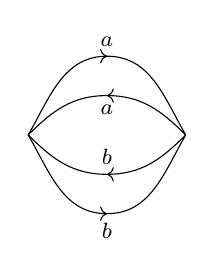
\begin{tikzpicture}
\begin{scope}[decoration={markings,mark=at position 0.5 with {\arrow{>}}}]
\draw[postaction={decorate}] (0,0) to [out=60,in=-180] (1,1) node [above] {\footnotesize $a$} to [out=0,in=120] (2,0);
\draw[postaction={decorate}] (0,0) to [out=-60,in=-180] (1,-1) node [below] {\footnotesize $b$} to [out=0,in=-120] (2,0);
\draw[postaction={decorate}] (2,0) to [out=135,in=0] (1,0.5) node [below] {\footnotesize $a$} to [out=-180,in=45] (0,0);
\draw[postaction={decorate}] (2,0) to [out=-135,in=0] (1,-0.5) node [above] {\footnotesize $b$} to [out=-180,in=-45] (0,0);
\end{scope}
\end{tikzpicture}
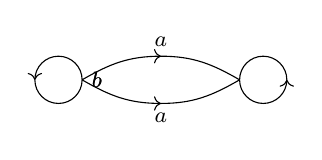
\begin{tikzpicture}
\begin{scope}[decoration={markings,mark=at position 0.5 with {\arrow{>}}}]
\draw[postaction={decorate}] (0,0) to [out=30,in=-180] (1,0.3) node [above] {\footnotesize $a$} to [out=0,in=150] (2,0);
\draw[postaction={decorate}] (0,0) to [out=-30,in=-180] (1,-0.3) node [below] {\footnotesize $a$} to [out=0,in=-150] (2,0);
\draw[postaction={decorate}] (-0.3,0) circle (0.3);
\node [right] (-0.6,0) {\footnotesize $b$};
\draw[postaction={decorate},rotate=180] (-2.3,0) circle (0.3);
\node [right] (2.6,0) {\footnotesize $b$};
\end{scope}
\end{tikzpicture}
\end{center}
\fi
And all connected $3$-sheeted coverings up to isomorphisms are \par
\vspace{3cm}
\textbf{Hatcher 1.3.12.} \par
Consider normal covering \par
\vspace{3cm}
Then $p_{*}(\pi_1(E,e))\leq \pi_1(B,b)$ is a normal subgroup, $a^2,b^2,(ab)^4\in p_{*}(\pi_1(E,e))$, and any element in $\pi_1(E,e)$ could be written as a product of $a^2,b^2,(ab)^4$, thus $p_{*}(\pi_1(E,e))$ is contained in the normal subgroup generated by $a^2,b^2,(ab)^4$, hence they are the same \par
\textbf{Hatcher 1.3.29.} \par
$p_1:Y\rightarrow Y/G_1, \, y\mapsto G_1y, \,p_2:Y\rightarrow Y/G_2, \, y\mapsto G_2y$ are both quotient and covering maps \par
If $G_2=gG_1g^{-1}$ are conjugate subgroups, for some $g\in \mathrm{Homeo}(Y)$, define $\overline{g}:Y/G_1 \rightarrow Y/G_2, \, G_1y\mapsto G_2gy $, it is well-defined since $\overline{g}(G_1gy)=G_2gg_1y=G_2g_2gy=G_2gy$ for some $g_2\in G_2$ such that $gg_1g^{-1}=g_2$ \par
Since, thus the following diagram commutes
\begin{center}
\begin{tikzcd}
& Y \arrow[r,"g"] \arrow[d,"p_1"] \arrow[dr,"p_2g"]
& Y \arrow[d,"p_2"] \\
& Y/G_1 \arrow[r,"\overline{g}"]
& Y/G_2
\end{tikzcd}
\end{center}
Also, $p_2g$ is continuous and $p_1$ is a quotient map, hence $\overline{g}$ is continunous \par
Similarly, define $\overline{g}^{-1}:Y/G_2\rightarrow Y/G_1, \, G_2y\mapsto G_1g^{-1}y$ is also continuous, then $\overline{g},\overline{g}^{-1}$ are inverses of each other, hence $\overline{g}:Y/G_1 \rightarrow Y/G_2$ is a homeomorphism \par
Conversely, suppose $\varphi:Y/G_1 \rightarrow Y/G_2$ is a homeomorphism, let $\psi=\varphi^{-1}$, Since $Y$ is path connected, locally path connected, simply connected, choose some $y_1,y_2\in Y$, such that $\varphi(G_1y)=G_2y$, then there exists a lift of $\varphi p_1$ against $p_2$, $\Phi:Y\rightarrow Y$ such that the following diagram commutes with $\Phi(y_1)=y_2$ \par
\begin{center}
\begin{tikzcd}
& Y \arrow[r,"\Phi"] \arrow[d,"p_1"]
& Y \arrow[d,"p_2"] \\
& Y/G_1 \arrow[r,"\varphi"]
& Y/G_2
\end{tikzcd}
\end{center}
Similarly, $\exists\Psi:Y\rightarrow Y$ such that the following diagram commutes with $\Psi(y_2)=y_1$ \par
\begin{center}
\begin{tikzcd}
& Y \arrow[d,"p_1"]
& Y \arrow[l,"\Psi"] \arrow[d,"p_2"] \\
& Y/G_1
& Y/G_2 \arrow[l,"\psi"]
\end{tikzcd}
\end{center}
Then $\Psi\Phi:Y\rightarrow Y$ is a deck transformation sending $y_1$ to $y_1$, thus $\Psi\Phi=\mathbbm{1}$, similarly, $\Phi\Psi=\mathbbm{1}$, hence $\Phi\in\mathrm{Homeo}(Y), \Psi=\Phi^{-1}$, we need to show $\Phi G_1\Phi^{-1}=G_2$ \par
$\forall y\in Y, \, G_2\Phi g_1\Phi^{-1}y=p_2\Phi g_1\Phi^{-1}y=\varphi p_1g_1\Phi^{-1}y=\varphi G_1g_1\Phi^{-1}y=\varphi G_1\Phi^{-1}y=\varphi p_1\Phi^{-1}y=p_2\Phi\Phi^{-1}y=p_2y=G_2y$ which implies $\Phi g_1\Phi^{-1}$ is a deck transformation of $p_2:Y\rightarrow Y/G_2$, hence $\Phi g_1\Phi^{-1}\in G_2 \Rightarrow \Phi G_1\Phi^{-1}\leq G_2$, similarly, $\Psi G_2\Psi^{-1}\leq G_1 \Rightarrow G_2 \leq\Phi G_1\Phi^{-1}$, thus $G_2 =\Phi G_1\Phi^{-1}$ \par
\textbf{1.} \par
Suppose $E_1\overset{p_1}{\rightarrow}B,\,E_2\overset{p_2}{\rightarrow}B$ are any two simply connected covers, $b=p_1(e_1)=p_2(e_2)$ for some $e_1\in E_1,e_2\in E_2$, then $\exists \Phi:E_1\rightarrow E_2$ with $\Phi(e_1)=e_2$ and $\exists \Psi:E_2\rightarrow E_1$ with $\Phi(e_2)=e_1$ such that the following diagram commutes \par
\begin{center}
\begin{tikzcd}
& E_1 \arrow[r,"\Phi"]\arrow[d,"p_1"]
& E_2 \arrow[r,"\Psi"]\arrow[d,"p_2"]
& E_1 \arrow[d,"p_1"] \\
& B & B & B
\end{tikzcd}
\end{center}
Thus $\Psi\Phi:E_1\rightarrow E_1$ sends $e_1$ to $e_1$, by the uniqueness of liftings, $\Psi\Phi=\mathbbm{1}$, similarly, $\Phi\Psi=\mathbbm{1}$, hence $E_1\overset{\Phi}{\rightarrow}E_2$ is a homeomorphism \par
\textbf{2.} \par
Denote the set of $G$-equivariant maps $G/H\rightarrow Y$ as $Y$ \par
Define $\varphi:Y\rightarrow X^H$, by $\varphi(f)=f(H)$, since $f$ is $G$-equivariant, $hf(H)=f(hH)=f(H)$, thus $f(H)\in X^H$ and also define $\psi:X^H\rightarrow Y$ by $\psi(x)=f$ where $f(gH)=gx$ is a $G$-equivariant map, it is obvious that $\varphi\psi=\psi\varphi=\mathbbm{1}$, we only need to show both $\varphi$ and $\psi$ are continuous \par
Let $X^{G/H}$ be the set of continuous functions from $G/H$ to $X$, $\{U\cup X^H\left|U \text{ open in } X\right.\}$ are the open sets of $X^H$, and $\displaystyle\bigcap_{i=1}^n\left\{f\in X^{G/H}\left|f(g_i(H))\in U_{g_iH}\right.\right\}$ form a basis for $X^{G/H}$, where $U_{g_iH}$ is just some open set in $X$ with $g_iH$ as its index \par
Thus
\[
\begin{aligned}
\bigcap_{i=1}^n\left\{f\in X^{G/H}\left|f(g_i(H))\in U_{g_iH}\right.\right\}\bigcap Y
&=\bigcap_{i=1}^n\left\{f\in Y\left|g_if(H)\in U_{g_iH}\right.\right\} \\
&=\bigcap_{i=1}^n\left\{f\in Y\left|f(H)\in g_i^{-1}U_{g_iH}\cap X^H\right.\right\}
\end{aligned}
\]
Form a basis for $Y$, Since
\[
\varphi\left(\left\{f\in Y\left|f(H)\in U\cap X^H\right.\right\}\right)\subseteq U\cap X^H
\]
And
\[
\psi\left(\bigcap_{i=1}^n g_i^{-1}U_{g_iH}\bigcap X^H\right)\subseteq\bigcap_{i=1}^n\left\{f\in Y\left|f(H)\in g_i^{-1}U_{g_iH}\cap X^H\right.\right\}
\]
$\varphi$ and $\psi$ are both continuous \par
\textbf{3.} \par
Let $X=\mathbb{R}\times I$ which is simply connected, define group action $\mathbb{Z}\times X\rightarrow X$ by $(n,(x,t))\mapsto f^n(x,t)$, then $p:X\rightarrow X/\mathbb{Z}$ is a universal cover \par
\textbf{(a)} \par
Since isomorphism classes of covering spaces are in one to one correspondence to conjugacy classes of subgroups, all path connected covering spaces of the Mobius band up to a covering isomorphism are $p_n:X/n\mathbb{Z}\rightarrow X/\mathbb{Z}, n\mathbb{Z}(x,t)\mapsto \mathbb{Z}(x,t)$, where $n=0,1,2\cdots$ , thus ${p_n}_{*}(X/n\mathbb{Z})=n\mathbb{Z}$\par
\textbf{(b)} \par
Since $m|n \Leftrightarrow {p_m}_{*}(X/m\mathbb{Z})=m\mathbb{Z}\leq n\mathbb{Z}={p_n}_{*}(X/n\mathbb{Z})$, hence all homomorphisms between these covering spaces are $\varphi_{n,m}:X/n\mathbb{Z}\rightarrow X/m\mathbb{Z}, n\mathbb{Z}(x,t)\mapsto m\mathbb{Z}(x,t)$

\end{document}